\documentclass[border=2pt]{standalone}
\usepackage{tikz}
\usetikzlibrary{arrows.meta}
\begin{document}
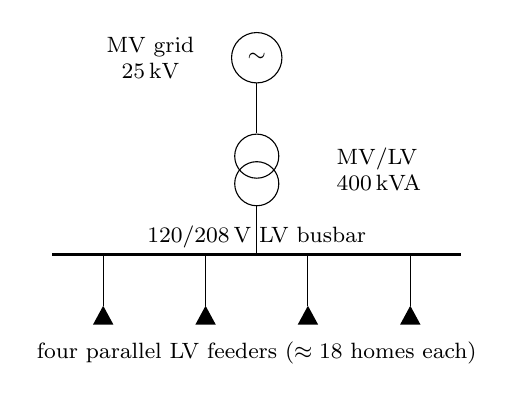
\begin{tikzpicture}[>=Latex, font=\footnotesize]
  \draw (0,0) circle (0.32) node {$\sim$};
  \node at (-1.35,0) [align=center] {MV grid\\25\,kV};
  \draw (0,-0.32) -- (0,-0.95);
  \draw (0,-1.25) circle (0.28);
  \draw (0,-1.60) circle (0.28);
  \node at (1.55,-1.42) [align=left] {MV/LV\\400\,kVA};
  \draw (0,-1.88) -- (0,-2.5);
  \draw[line width=1.1pt] (-2.6,-2.5) -- (2.6,-2.5);
  \node at (0,-2.27) {120/208\,V LV busbar};
  \foreach \x in {-1.95,-0.65,0.65,1.95}{
     \draw (\x,-2.5) -- (\x,-3.15);
     \fill (\x,-3.15) -- ++(-0.13,-0.24) -- ++(0.26,0) -- cycle;
  }
  \node at (0,-3.75) [align=center]
    {four parallel LV feeders ($\approx 18$ homes each)};
\end{tikzpicture}
\end{document}
